	\addtolength{\oddsidemargin}{-.875in}
	\addtolength{\evensidemargin}{-.875in}
	\addtolength{\textwidth}{1.75in}

	\addtolength{\topmargin}{-.875in}
	\addtolength{\textheight}{1.75in}

\twocolumn[

\begin{@twocolumnfalse}
    \maketitle
    \begin{abstract}
      Hello I am the abstract,here are a bunch of words so we can see the full width and check that the style our fantastic creator has made is satisfactory
    \end{abstract}
  \end{@twocolumnfalse}
]

\begin{thebibliography}{9}

\bibitem{textbook}
Y. Shoham and K. Leyton-Brown, Multiagent systems. Cambridge: Cambridge Univ. Press, 2012.

\bibitem{RL}
Pineau and N. Roy, "Reinforcement learning with limited reinforcement: Using Bayes risk for active learning in POMDPs", Artificial Intelligence, vol. 187-188, pp. 115-132, 2012. Available: 10.1016/j.artint.2012.04.006.

\bibitem{Vickrey}
W. Vickrey, "Counterspeculation, Auctions, and Competitive Sealed Tenders", The Journal of Finance, vol. 16, no. 1, p. 8, 1961. Available: 10.2307/2977633.

\bibitem{RLtextbook}
S. Russell and P. Norvig, Artificial intelligence.

\end{thebibliography}

\appendix[Assignment and Game details (on next page)]

\begin{figure*}[!h]
\centering
\subfloat{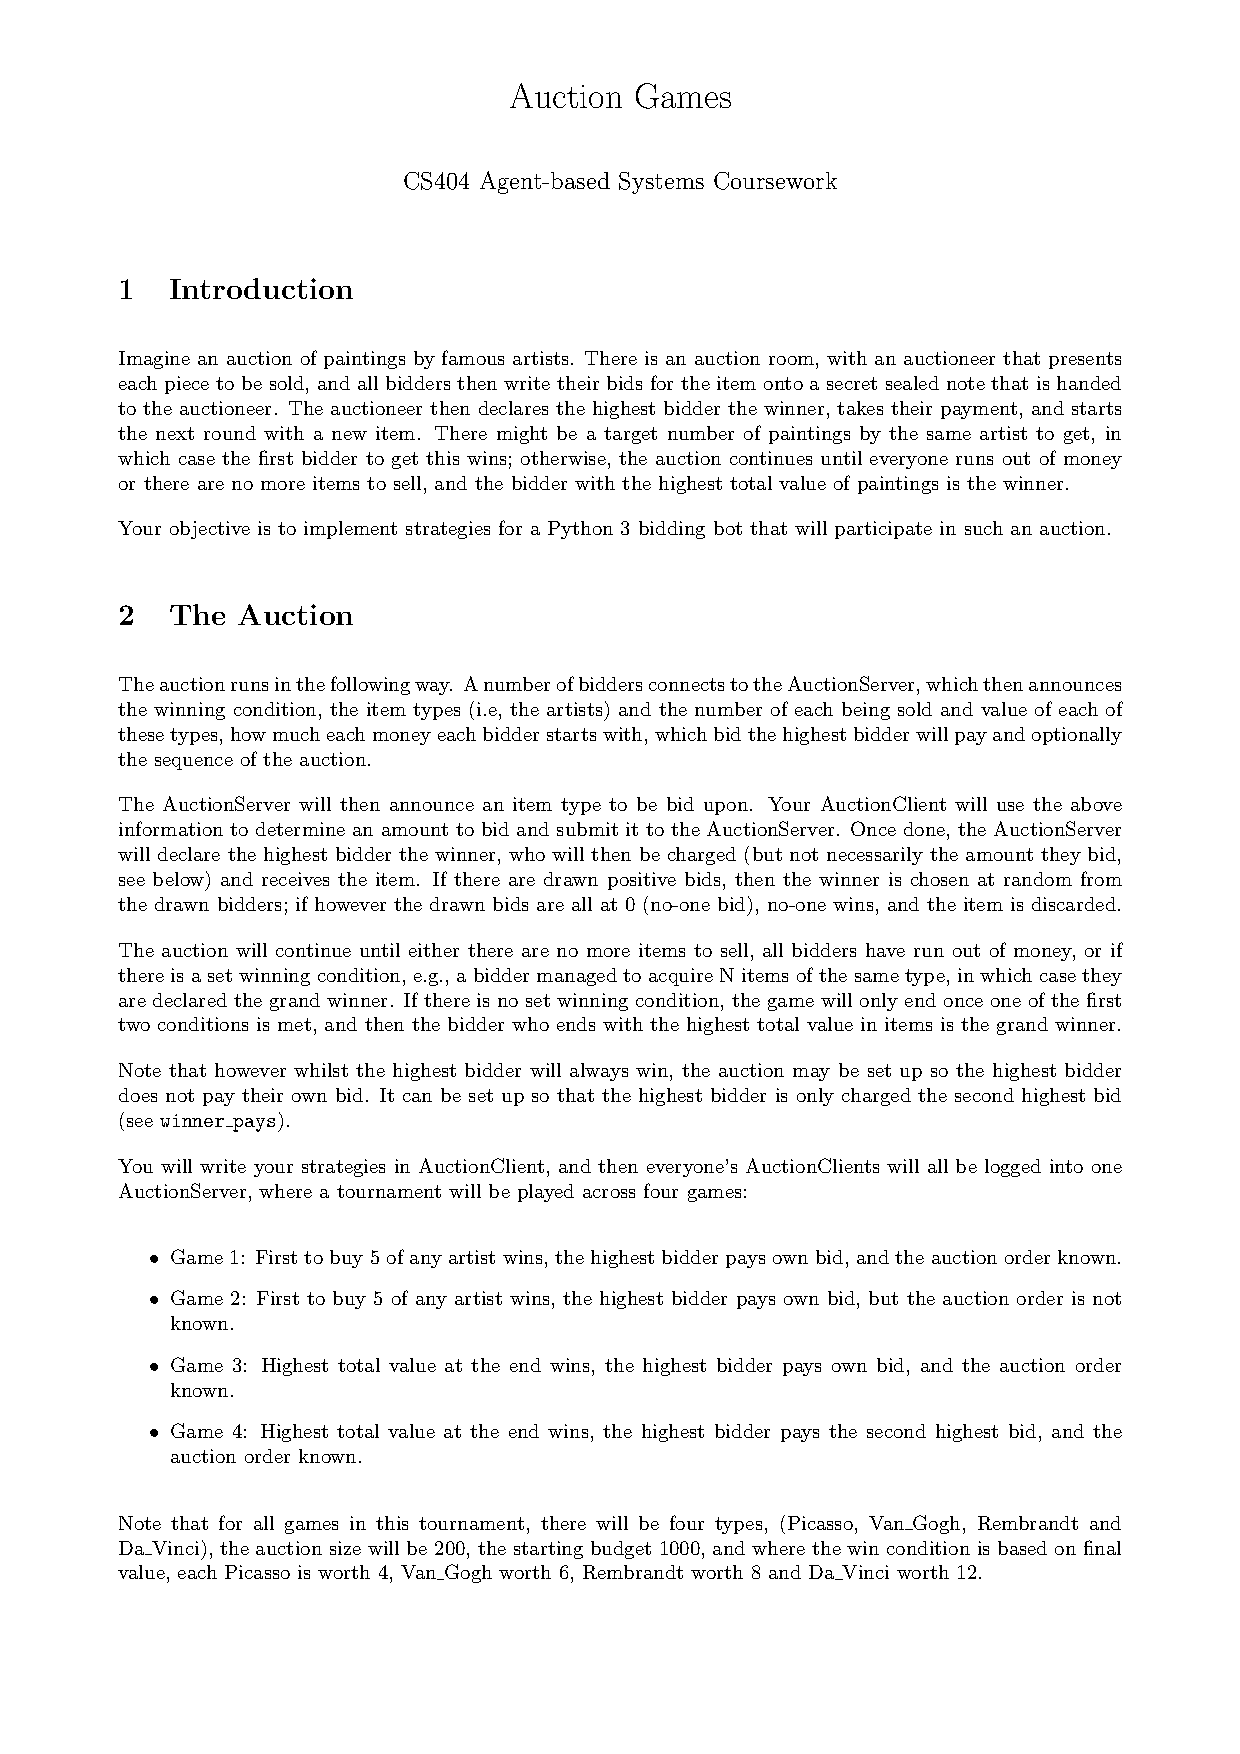
\includegraphics[page=1,width=0.5\textwidth]{spec19.pdf}}
\hfil
\subfloat{\includegraphics[page=2,width=0.5\textwidth]{spec19.pdf}}
\subfloat{\includegraphics[page=3,width=0.5\textwidth]{spec19.pdf}}
\end{figure*}